\cmfnewsection{Automação de Simulações}{./logos/fundo_tese}{0.15}





%%%%%%%%%%%%%%%%%%%%%%%%%%%%%%%%%%%%%%%%%%%%%%%%
%%%%%%%%%%%%%%%%%%%%%%%%%%%%%%%%%%%%%%%%%%%%%%%%
%%%%%%%%%%%%%%%%%%%%%%%%%%%%%%%%%%%%%%%%%%%%%%%%
%%%%%%%%%%%%%%%%%%%%%%%%%%%%%%%%%%%%%%%%%%%%%%%%
\begin{frame}{O que significa automatizar simulações?}
\centering


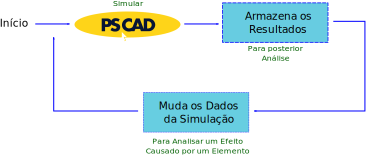
\includegraphics[width=0.80\linewidth]{./figuras/Automacao/automa}


\end{frame}





%%%%%%%%%%%%%%%%%%%%%%%%%%%%%%%%%%%%%%%%%%%%%%%%
%%%%%%%%%%%%%%%%%%%%%%%%%%%%%%%%%%%%%%%%%%%%%%%%
%%%%%%%%%%%%%%%%%%%%%%%%%%%%%%%%%%%%%%%%%%%%%%%%
%%%%%%%%%%%%%%%%%%%%%%%%%%%%%%%%%%%%%%%%%%%%%%%%
\begin{frame}{Por que automatizar simulações?}
\centering

\textbf{Motivo 1:} Ajustar sistemas de controle
\vspace*{0.5cm}

\includegraphics[width=0.55\linewidth]{./figuras/Automacao/SISTEMA}

\end{frame}







%%%%%%%%%%%%%%%%%%%%%%%%%%%%%%%%%%%%%%%%%%%%%%%%
%%%%%%%%%%%%%%%%%%%%%%%%%%%%%%%%%%%%%%%%%%%%%%%%
%%%%%%%%%%%%%%%%%%%%%%%%%%%%%%%%%%%%%%%%%%%%%%%%
%%%%%%%%%%%%%%%%%%%%%%%%%%%%%%%%%%%%%%%%%%%%%%%%
\begin{frame}{Por que automatizar simulações?}
\centering

\textbf{Motivo 2:} Avaliar efeitos de eventos em diferentes pontos em um sistema grande\footnote[frame]{\tiny Verônica Rodrigues Feijão, \href{https://drive.google.com/file/d/1xZGZLela_iNW0KIjTQ59YyCL1-sb16IO/view}{Estudo de Localização de Faltas de Curta Duração para uma Rede de 14 Barras}. Projeto de Graduação -  UERJ, 2019.}
%\vspace*{1cm}

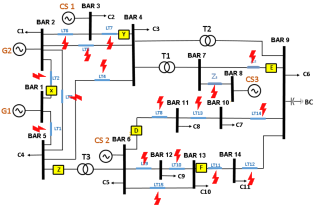
\includegraphics[width=0.6\linewidth]{./figuras/Automacao/ex_curto}

\end{frame}





%%%%%%%%%%%%%%%%%%%%%%%%%%%%%%%%%%%%%%%%%%%%%%%%
%%%%%%%%%%%%%%%%%%%%%%%%%%%%%%%%%%%%%%%%%%%%%%%%
%%%%%%%%%%%%%%%%%%%%%%%%%%%%%%%%%%%%%%%%%%%%%%%%
%%%%%%%%%%%%%%%%%%%%%%%%%%%%%%%%%%%%%%%%%%%%%%%%
\begin{frame}{Como fazer?}
\centering

\begin{columns}


\column{0.5\linewidth}

\begin{itemize}
\item Inserir/Configurar o bloco {\it Multiple run} localizado no grupo de {\it I/O Devices} na biblioteca Master.

\vspace*{2.5cm}

\item Configurar o projeto para {\it Multiple run}.

\vspace*{1cm}
\end{itemize}


\column{0.5\linewidth}
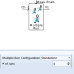
\includegraphics[width=0.80\linewidth]{./figuras/Automacao/multrun}

\end{columns}

\end{frame}




%%%%%%%%%%%%%%%%%%%%%%%%%%%%%%%%%%%%%%%%%%%%%%%%
%%%%%%%%%%%%%%%%%%%%%%%%%%%%%%%%%%%%%%%%%%%%%%%%
%%%%%%%%%%%%%%%%%%%%%%%%%%%%%%%%%%%%%%%%%%%%%%%%
%%%%%%%%%%%%%%%%%%%%%%%%%%%%%%%%%%%%%%%%%%%%%%%%
\begin{frame}{Circuito Exemplo}
\centering

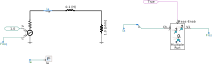
\includegraphics[width=0.85\linewidth]{./figuras/Automacao/SIM}

\end{frame}